\documentclass[aspectratio=169]{beamer}
\usetheme{Madrid}
\usecolortheme{default}

\usepackage{fontspec}
\usepackage{polyglossia}
\setmainlanguage{spanish}
\usepackage{graphicx}
\usepackage{amsmath}
\usepackage{booktabs}
\usepackage{xcolor}

\definecolor{ejemplocolor}{RGB}{180,83,9}

\setbeamertemplate{navigation symbols}{}
\setbeamertemplate{footline}[frame number]
\setbeamerfont{footnote}{size=\tiny}

\newcommand{\fuente}[1]{{\footnotesize\textit{Fuente: #1}}}
\newcommand{\ejemplo}[1]{\par\vspace{0.4em}{\small\color{ejemplocolor}\textbf{Ejemplo:} #1}}

\title[1. Fundamentos]{Capítulo 1: Fundamentos del\\Aprendizaje Automático}
\subtitle{Material del curso}
\author{Universidad de Salamanca}
\institute{Facultades de Ciencias y Ciencias Químicas}
\date{\today}

\begin{document}

% ============================================================
\begin{frame}
  \titlepage
\end{frame}

\begin{frame}{En este capítulo}
  \begin{enumerate}
    \item \textbf{1.1 Historia y evolución} del aprendizaje automático
    \begin{itemize}
      \item De los mínimos cuadrados (1805) a la IA Generativa
      \item Los ``inviernos de la IA'' y por qué ocurrieron
    \end{itemize}
    \item \textbf{1.2 Conceptos fundamentales}
    \begin{itemize}
      \item Datos, \textit{features} y etiquetas
      \item \textit{Overfitting}, validación cruzada y métricas
      \item El \textit{pipeline} de ML de principio a fin
    \end{itemize}
  \end{enumerate}
  \vspace{0.5em}
  Estos fundamentos son la base para todo lo que viene después: sin ellos, es difícil entender por qué un modelo funciona o falla.
\end{frame}

% ============================================================
\section{1.1 Historia y evolución}

\begin{frame}{¿Por qué aprender aprendizaje automático?}
  \begin{itemize}
    \item En programación \textbf{tradicional}, un humano escribe todas las reglas a mano:
    \begin{itemize}
      \small
      \item \texttt{si temperatura > 30: encender\_aire\_acondicionado()}
    \end{itemize}
    \item Pero muchos problemas son demasiado complejos para reglas fijas
    \item El \textbf{aprendizaje automático invierte el paradigma}: en vez de escribir las reglas, se le enseña a la máquina a \textit{aprender} las reglas a partir de ejemplos
  \end{itemize}
  \ejemplo{nadie puede escribir a mano una regla que distinga un gato de un perro en una foto, pero un modelo puede \textit{aprenderla} viendo miles de fotos ya etiquetadas.}
\end{frame}

\begin{frame}{El nuevo paradigma de programación}
  \begin{itemize}
    \item Para que una máquina aprenda hacen falta \textbf{tres elementos}:
    \begin{enumerate}
      \item Datos de entrada
      \item Ejemplos de la salida esperada (\textbf{etiquetas})
      \item Una forma de medir si lo está haciendo bien (\textbf{función de pérdida})
    \end{enumerate}
    \item La IA no es un concepto nuevo: convive con la IA simbólica (reglas lógicas escritas a mano), que dominó el campo entre los años 50 y finales de los 80
  \end{itemize}
\end{frame}

\begin{frame}{Raíces matemáticas y el Test de Turing (1805-1950)}
  \begin{columns}
    \begin{column}{0.6\textwidth}
      \begin{itemize}
        \item 1805: Legendre y Gauss publican los \textbf{mínimos cuadrados} --- la forma más temprana de regresión lineal
        \item 1936: Fisher propone el análisis discriminante lineal
        \item 1943: McCulloch y Pitts presentan el primer modelo de neurona artificial
        \item 1950: Alan Turing publica \textit{``Computing Machinery and Intelligence''} e introduce el \textbf{Test de Turing}
      \end{itemize}
    \end{column}
    \begin{column}{0.35\textwidth}
      \centering
      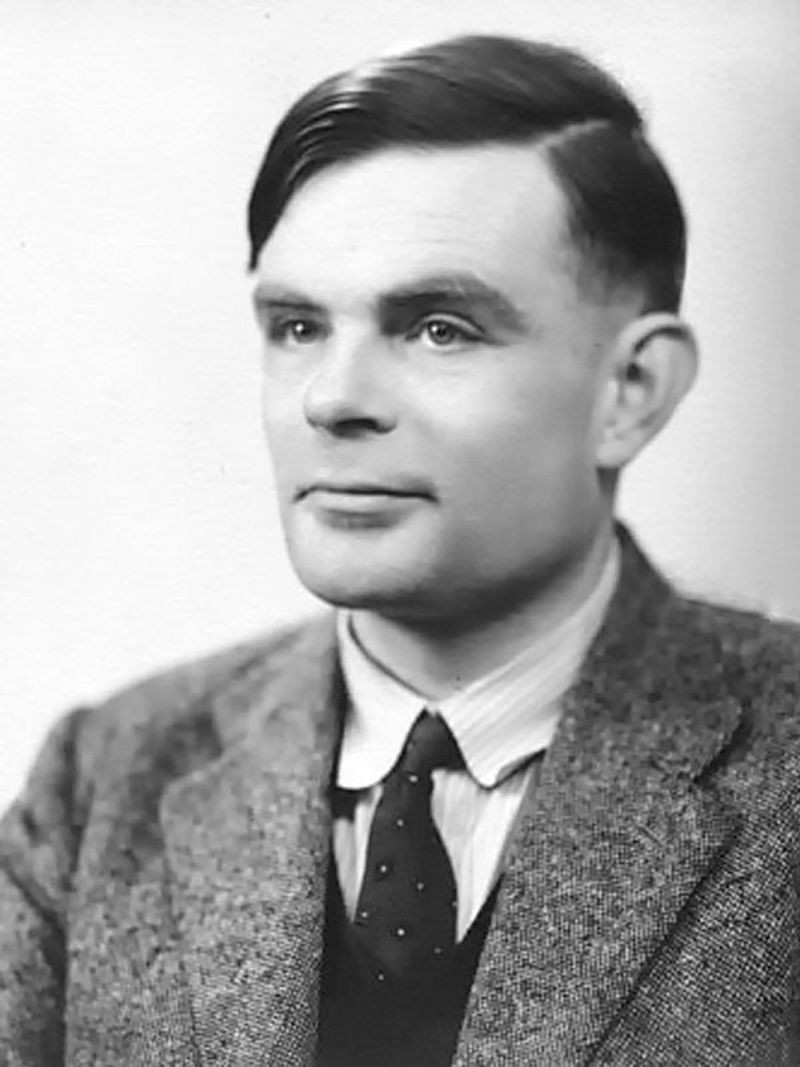
\includegraphics[width=0.85\textwidth]{../book/_static/external_images/alan_turing_1951.jpg}\\[0.3em]
      {\tiny\textit{Fuente: Elliott \& Fry (1951), dominio público}}
    \end{column}
  \end{columns}
\end{frame}

\begin{frame}{El nacimiento formal y la era simbólica (1956-1980)}
  \begin{itemize}
    \item 1956: John McCarthy organiza el \textbf{seminario de Dartmouth} --- nace formalmente la IA como campo de investigación
    \item Durante décadas se creyó que bastaría con codificar a mano un conjunto masivo de reglas lógicas (\textbf{IA simbólica})
    \item Este enfoque alcanzó su auge con los \textbf{sistemas expertos} en los años 80
  \end{itemize}
  \ejemplo{un sistema experto médico de los años 80 contenía miles de reglas del tipo ``si fiebre y tos y dolor de pecho, entonces sospechar neumonía'', escritas a mano por médicos.}
\end{frame}

\begin{frame}{El Perceptrón y los inviernos de la IA}
  \begin{columns}
    \begin{column}{0.6\textwidth}
      \begin{itemize}
        \item 1958: Frank Rosenblatt crea el \textbf{Perceptrón}, el primer modelo entrenable de neurona artificial
        \item \textbf{Primer invierno} (años 70): el Perceptrón no puede resolver problemas no lineales; el entusiasmo se desploma
        \item \textbf{Segundo invierno} (años 90): los sistemas expertos resultan caros de mantener, difíciles de escalar y limitados
        \item El ML despega de verdad en los 90, gracias a hardware más rápido y más datos disponibles
      \end{itemize}
    \end{column}
    \begin{column}{0.35\textwidth}
      \centering
      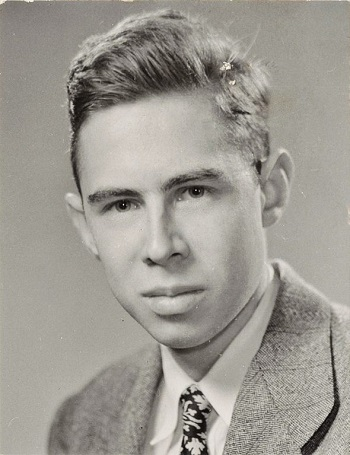
\includegraphics[width=\textwidth]{../book/_static/external_images/frank_rosenblatt.jpg}\\
      \fuente{Heinz Nixdorf MuseumsForum, CC BY-SA 4.0}
    \end{column}
  \end{columns}
\end{frame}

\begin{frame}{Línea temporal completa}
  \footnotesize
  Ciclos de ``verano'' (avances, financiación) e ``invierno'' (desilusión, recortes de fondos).
  \begin{center}
    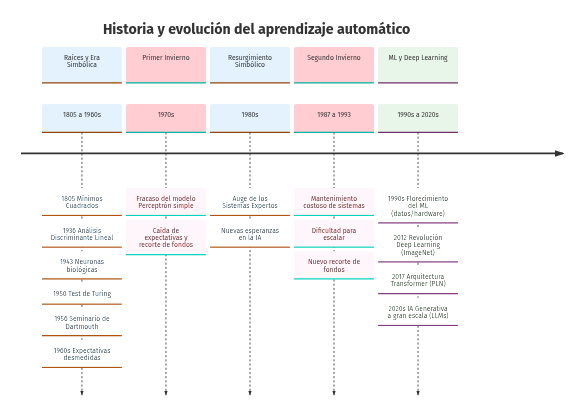
\includegraphics[width=0.62\textwidth]{../book/_static/generated/diagrams_pdf/es/00_fundamentos_01_historia_evolucion_01.png}
  \end{center}
\end{frame}

\begin{frame}{Del \textit{Deep Learning} a la era de los LLM (2010-hoy)}
  \begin{itemize}
    \item El \textbf{Aprendizaje Profundo} (\textit{Deep Learning}) aprende representaciones en capas sucesivas, cada vez más útiles para la tarea
    \item 2012: la victoria de Hinton en el desafío \textbf{ImageNet} marca el punto de inflexión
    \item \textbf{MNIST} (dígitos manuscritos 0-9) se convierte en el banco de pruebas clásico
    \item 2017: la arquitectura \textbf{Transformer} revoluciona el procesamiento de lenguaje natural
    \item 2020s: la \textbf{IA Generativa} (ChatGPT, Gemini) escala a miles de millones de parámetros
  \end{itemize}
  \begin{center}
    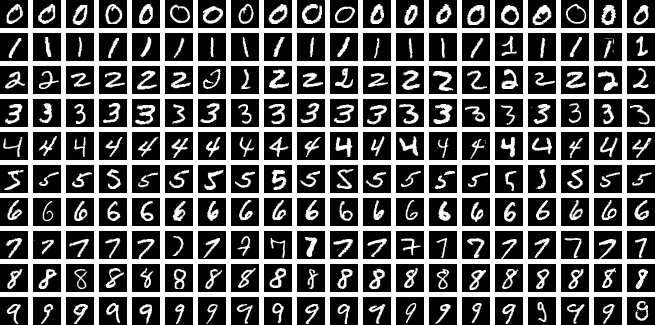
\includegraphics[width=0.42\textwidth]{../book/_static/external_images/mnist_dataset_example.png}\\
    \fuente{Suvanjanprasai (2024), Wikimedia Commons, CC BY-SA 4.0}
  \end{center}
\end{frame}

\begin{frame}{Resumen: 1.1 Historia y evolución}
  \begin{itemize}
    \item El ML nació de una pregunta: ¿pueden las máquinas aprender?
    \item Ha pasado por ciclos de entusiasmo (\textit{hype}) y desencanto
    \item Los avances recientes vienen de más datos, mejor hardware y algoritmos nuevos
    \item El \textit{Deep Learning} y los LLM son el estado del arte actual
  \end{itemize}
\end{frame}

% ============================================================
\section{1.2 Conceptos fundamentales}

\begin{frame}{Datos, \textit{features} y etiquetas}
  \begin{center}
    \begin{tabular}{lcccc}
      \toprule
      Muestra & Feature 1 & Feature 2 & Feature 3 & Label \\
      \midrule
      1 & 25 & 70 & 175 & Gato \\
      2 & 8 & 4 & 90 & Gato \\
      3 & 35 & 80 & 180 & Perro \\
      \bottomrule
    \end{tabular}
  \end{center}
  \vspace{0.5em}
  \begin{itemize}
    \item \textbf{Muestra}: un punto de datos individual (una fila de la tabla)
    \item \textbf{\textit{Features}}: los atributos que describen la muestra
    \item \textbf{Etiqueta}: lo que queremos predecir --- la ``verdad fundamental''
  \end{itemize}
  \ejemplo{para predecir el precio de una vivienda, las \textit{features} serían m\textsuperscript{2}, número de habitaciones y ubicación; la etiqueta sería el precio.}
\end{frame}

\begin{frame}{\textit{Overfitting} vs. \textit{underfitting}}
  \begin{itemize}
    \item \textbf{\textit{Underfitting}} (alto sesgo): el modelo es demasiado simple, no capta el patrón real
    \item \textbf{\textit{Overfitting}} (alta varianza): el modelo memoriza el ruido de entrenamiento en vez de aprender la tendencia
    \item El objetivo es el equilibrio sesgo-varianza que mejor generaliza a datos nuevos
  \end{itemize}
  \ejemplo{es como estudiar para un examen memorizando las respuestas exactas de un simulacro (\textit{overfitting}) en vez de entender el tema: fallarás en cuanto cambien las preguntas.}
  \begin{center}
    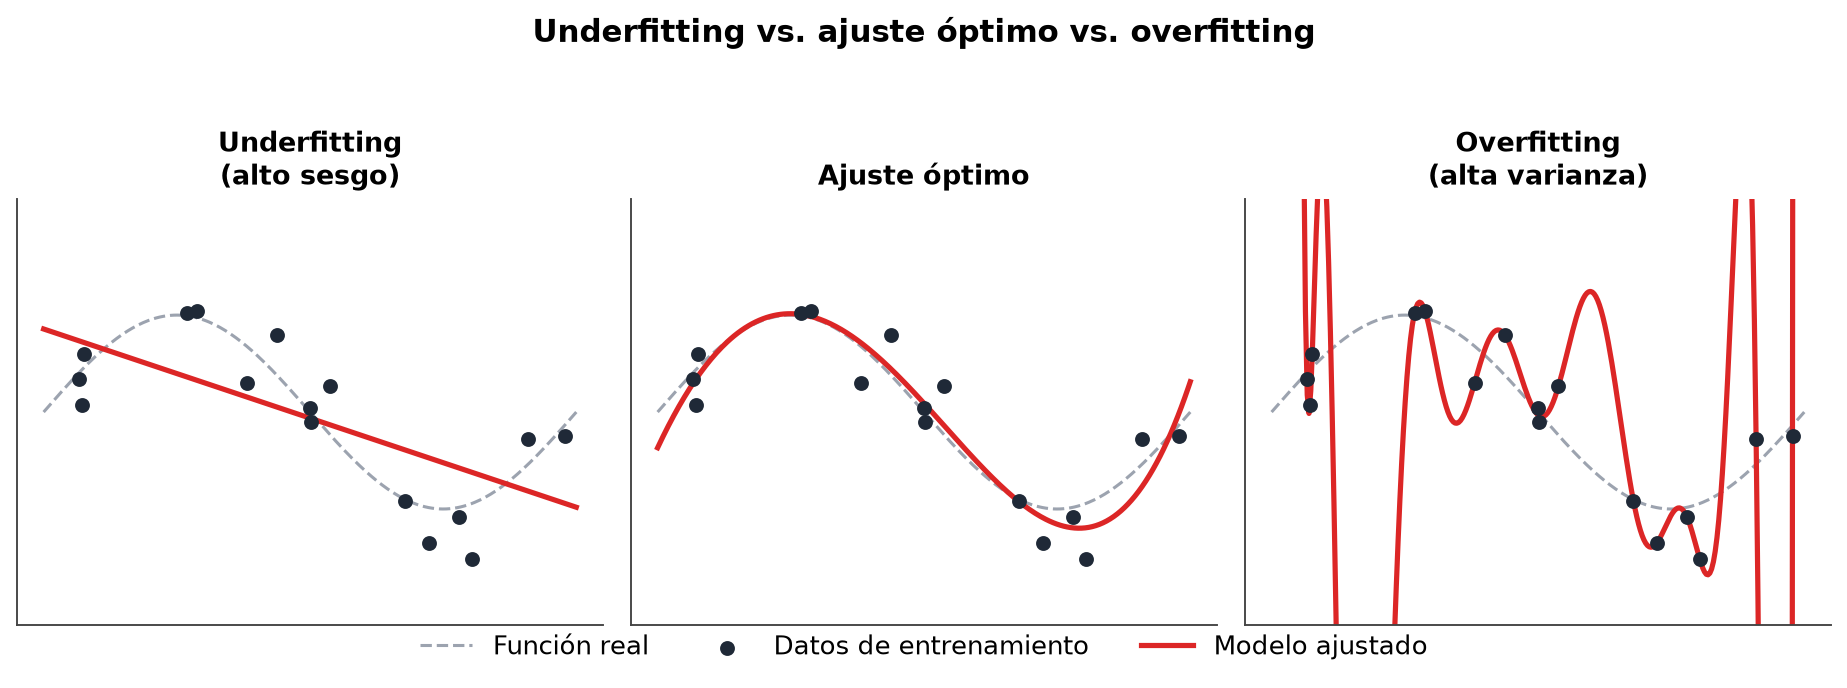
\includegraphics[width=0.62\textwidth]{../book/_static/generated/figures/es/overfitting_underfitting.png}
  \end{center}
\end{frame}

\begin{frame}{Validación cruzada $K$-\textit{fold}}
  \begin{itemize}
    \item División estándar: \textbf{entrenamiento} (ajustar pesos), \textbf{validación} (elegir hiperparámetros) y \textbf{prueba} (evaluación final imparcial)
    \item $K$-\textit{fold}: se divide en $K$ partes; se entrena $K$ veces usando cada vez una parte distinta como validación
    \item La métrica final es la media de los $K$ resultados --- reduce la varianza de la estimación
    \item \textbf{Estratificación}: cada partición debe conservar la proporción de clases del conjunto original
  \end{itemize}
  \begin{center}
    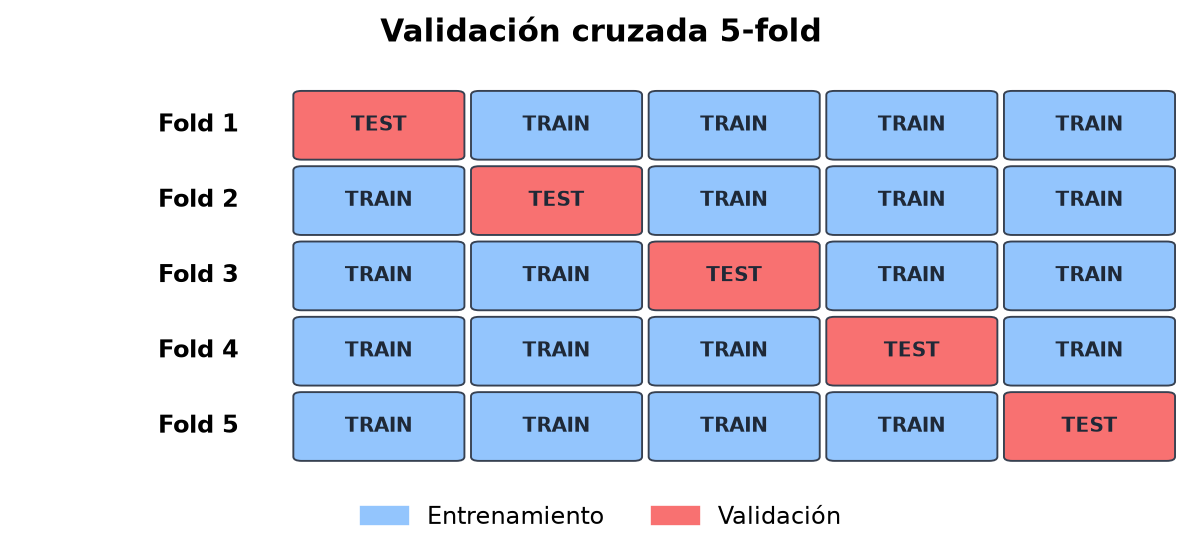
\includegraphics[width=0.55\textwidth]{../book/_static/generated/figures/es/kfold_cross_validation.png}
  \end{center}
\end{frame}

\begin{frame}{Matriz de confusión y métricas}
  \begin{columns}
    \begin{column}{0.48\textwidth}
      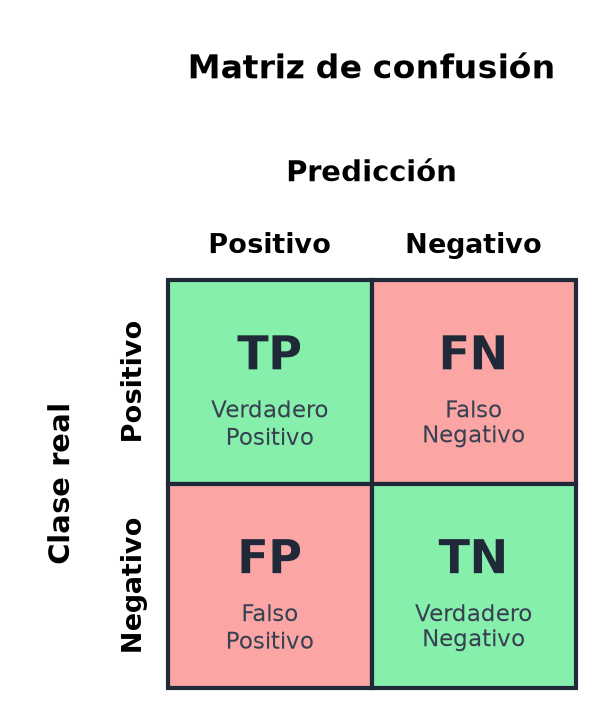
\includegraphics[width=0.75\textwidth]{../book/_static/generated/figures/es/confusion_matrix.png}
    \end{column}
    \begin{column}{0.5\textwidth}
      \footnotesize
      \begin{align*}
        \text{Precisión} &= \frac{TP}{TP+FP} \\
        \text{Recall} &= \frac{TP}{TP+FN} \\
        F1 &= 2\cdot\frac{P \times R}{P + R}
      \end{align*}
    \end{column}
  \end{columns}
  \ejemplo{\footnotesize en un diagnóstico médico, un \textbf{falso negativo} (decir ``sano'' a un paciente enfermo) suele ser más grave que un falso positivo. Por eso a veces se prioriza el \textit{recall} sobre la precisión.}
\end{frame}

\begin{frame}{El \textit{pipeline} de ML: 10 etapas}
  \begin{columns}
    \begin{column}{0.4\textwidth}
      \footnotesize
      \begin{itemize}
        \item Proceso \textbf{iterativo}: la evaluación puede obligar a volver a etapas anteriores
        \item Gran parte del esfuerzo real está en las etapas 2-3 (datos) y 7-8 (ajuste)
        \item El despliegue no es el final: requiere monitorización continua, porque los datos reales cambian con el tiempo (\textit{concept drift})
      \end{itemize}
    \end{column}
    \begin{column}{0.57\textwidth}
      \centering
      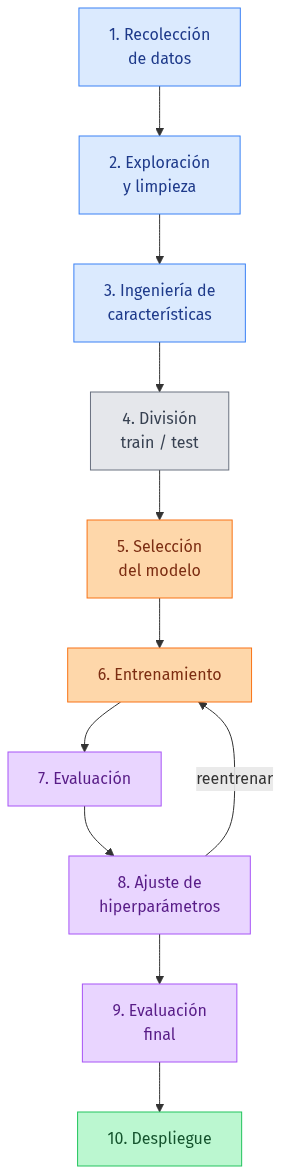
\includegraphics[height=0.75\textheight]{../book/_static/generated/diagrams_pdf/es/00_fundamentos_02_conceptos_fundamentales_01.png}
    \end{column}
  \end{columns}
\end{frame}

\begin{frame}{Resumen: 1.2 Conceptos fundamentales}
  \begin{itemize}
    \item \textbf{Muestra / \textit{feature} / etiqueta}: las piezas básicas de cualquier dataset
    \item \textbf{\textit{Overfitting} / \textit{underfitting}}: la tensión central del aprendizaje automático
    \item \textbf{Validación cruzada}: evaluar sin sesgo cuando los datos escasean
    \item \textbf{Métricas}: elegir la adecuada según lo que importe (precisión o \textit{recall})
    \item \textbf{\textit{Pipeline} de ML}: 10 etapas, de la recolección de datos al despliegue
  \end{itemize}
\end{frame}

\begin{frame}
  \centering
  {\Huge Fin del Capítulo 1}\\[1em]
  {\large Siguiente: Capítulo 2 --- Aprendizaje Supervisado}
\end{frame}

\end{document}
